\chapter{Data Cleaning for the Five Station Analysis}

  The data taken by the Askaryan Radio Array have been analyzed a few times for neutrinos, solar flares, and to deduce the properties of the ice at the South Pole. 
  When the livetime of the five stations is added together, there are roughly 28 station-years of data but only 9 years of that data have been analyzed.
  This is partly because each station takes so long to calibrate and prepare for analysis but also because there is so much data to clean before one can perform an analysis. 
  For example, 8 of the station years that have been analyzed were analyzed by a team lead by two graduate students. 
  ARA currently has 5 graduate students, 2 postdoctoral researchers, and a faculty member who are devoted to analyzing the full 28 station-years of ARA data. 
  This process involves building an analysis pipeline from the ground up, cleaning years of data, and simulating neutrino and noise events then viewing how many are removed through the cleaning pipeline, and analyzing remaining events for neutrino signals. 
  
\section{Simulation Setup for Data Cleaning}

  It is important to consider how each cut translates to overall data loss and expected neutrino event data loss. 
  Neutrino events are therefore simulated uniformly in log( energy ) space with energies from $10^{15}$ eV to $10^{21}$ eV. 
  As in Chapter 4 Section 4, neutrinos are thrown in a forward simulation along trajectories that intersect with a cylinder 15~km in radius and 3~km in depth. % Fix this reference, use variables
  These neutrinos interact randomly within the Earth and all outgoing particles with energy greater than $10^{16}$ eV are simulated further. 
  Muon and tau stochastic losses, tau decays, and outgoing neutrino interactions are simulated. 
  
  Noise simulations are also generated using the spectral coefficients calculated from the "software trigger" events that are read out once per second, regardless of sufficient signal to trigger the detector. % Check the frequency of these events
  \missingfigure{Noise spectral coefficients for A2}
  \missingfigure{Example of a software trigger event and a simulated noise event.}
  
  The traces of the signal simulations and noise simulations are fed through the cleaning pipeline so that, as cuts are applied to remove backgrounds from the dataset, we can ensure that we are doing so in a way that maximized the potential residual neutrino event population. 
  At the end of data cleaning, the goal is that our data distributions for key analysis variables resemble the noise simulation distributions such that any outliers that may arise are due to neutrino events. 
  
\section{Defining Livetime Configurations for A2 \label{sec:a2configs}}

  The behavior of detector triggering and readout changes dramatically as the detector's configuration is changed. 
  This has serious effects on event reconstruction and analysis, so each station's livetime is divided into livetime configurations. 
  These livetime configurations are mostly based on antenna/string masking, trigger window, and the amount of waveform readout ahead of the bin that triggered the detector, called the pre-trigger readout window or the number of pre-RF blocks. 
  Each trigger block is 10~ns and the total trigger window is defined as 
  \begin{equation}
    TW = (N_{TB}+1) * 10~\text(ns)
    \ref{eq:trigwin}
  \end{equation}
  and the default trigger window is 10 blocks meaning 110~ns.
  Each RF block is 20~ns and the default setting for pre-RF blocks is 10, so the default pre-trigger readout window is 200~ns. 
  As a station needs three like-polarization antennas to trigger, there may be signal recorded one or more antennas in advance of the bin that triggered so it's important to tune the number of pre-RF blocks accordingly. 
  Having too few pre-RF blocks yielded poor reconstruction of calibration pulser events in configuration 6 of station 2 after String 1 was masked and was noticed in June 2020 on an Operations Call and adjusted. 
  \missingfigure{Examples of Calpulser events in A2C5, C6, and C7}
  \missingfigure{Reconstructed calpulser vs unixtime to show deterioration in C6}
  
  Figure~\ref{fig:configs} shows the evolution of these key parameters for the full station 2 livetime along with shaded regions indicating each defined livetime configuration. 
  What is not pictured in this figure is the masking of String 1 of Station 2 which began on run 15527 in January of 2020. 
  Note that these configurations have changed since the 4 year survey of Stations 2 and 3. 
  That analysis placed emphasis on the masked antennas, trigger window, presence of trigger delays, and full readout window length. 
  This analysis has discovered that the latter 2 settings are less impactful when defining run configurations compared to the antenna masking, trigger window, and recently appreciated pre-trigger readout window. 
  Further considering each new livetime configuration requires a distinct set of noise, signal, and effective volume simulations that take well over a hundred thousand CPU-hours to generate, livetime configuration permutations are minimized by only considering the trigger window, pre-trigger readout window, and the status of antenna masking. 
  \missingfigure{trigger window and pre RF blocks over time for A2 \label{fig:configs}}
  \missingfigure{Table of the configs like the one on the Wiki}
  
\section{Using the AraProc Analysis Pipeline}

  AraProc is a python-based framework spearheaded by Dr Marco Muzio and Professor Brian Clark that reads in L1 ARA data and converts it into condensed L2 data. % Provide the link
  The root-formatted L1 data include raw waveforms that take up roughly 7 GB of space per full run. 
  The root-formatted L2 data is created using the L1 data but only includes simple metadata and analysis variables describing each event, so full runs of L2 data only take up roughly 6 MB of space. 
  The preexisting metadata saved includes the time of an event, the trigger type, and the detector configuration among other settings. 
  The calculated analysis variables generated by AraProc include the reconstructed azimuth, zenith, and signal correlation for nearby "pulser" maps and distant 300m maps for each polarization (horizontal and vertical) as well as direct and refracted rays for the distant maps. 
  The radius of the pulser map used for the reconstruction is uniquely set to the physical distance from a station's pulser to the station's center.
  Other analysis variables include the SNR of the coherently summed waveform for an event, the average RMS of the waveforms, the impulsivity, and the spark power ratios. 
  Some of these analysis variables will be explained in more detail in the coming sections as they are used to employ various cuts. 
  The AraProc framework can be run on computing clusters so many runs may be processed in parallel. 
  \todo{Showcase some of the analysis variables}
  
\section{Removing Spoiled Data}

  The first genre of cuts that will be discussed are those that remove bad events from the data. 
  These events are usually the result of digitizing malfunctions. 
  
  \subsection{1st Minute Cut}
  
    During the first minute of a run, events from ARA stations are typically corrupted as the waveforms recorded usually have a large offset compared to the pedestal values of the waveform. 
    This is the result of unstable power draw in the station as it starts a new run. 
    Due to this large offset, it is expected that the average waveform RMS and SNR are abnormal during the first minute of a run compared to the remainder of the run. 
    Shown in Figure~\ref{fig:firstmin_waveform} are the waveforms in every ARA2 channel for an event in the first minute of a run. 
    Figure~\ref{fig:firstmin_2d} shows how the average waveform RMS changes in the first 10 minutes of a run as well. 
    The impulsive nature of these waveforms can mimic the neutrino signal this analysis is targeting so these events must be removed from the analysis. 
    
    
    \begin{figure}
      \centering
      \begin{subfigure}[t]{0.48\textwidth}
        \centering
        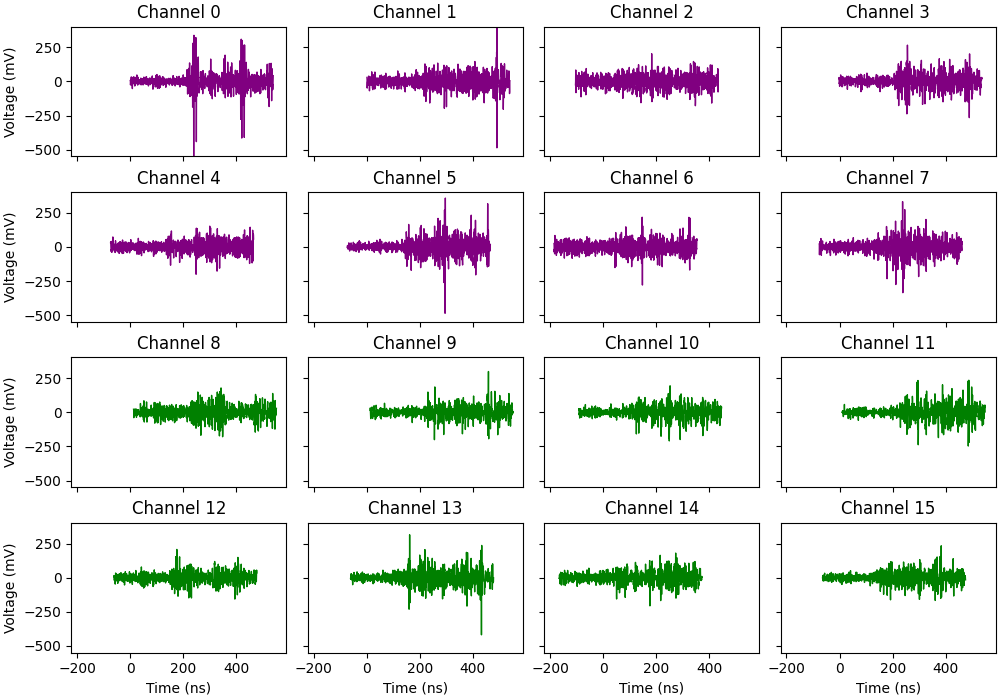
\includegraphics[width=\textwidth]{sections/5sa-cleaning/images/firstmin_station_2_run_17627_eventNo_2_trace.png}
      \end{subfigure}
      ~
      \begin{subfigure}[t]{0.48\textwidth}
        \centering
        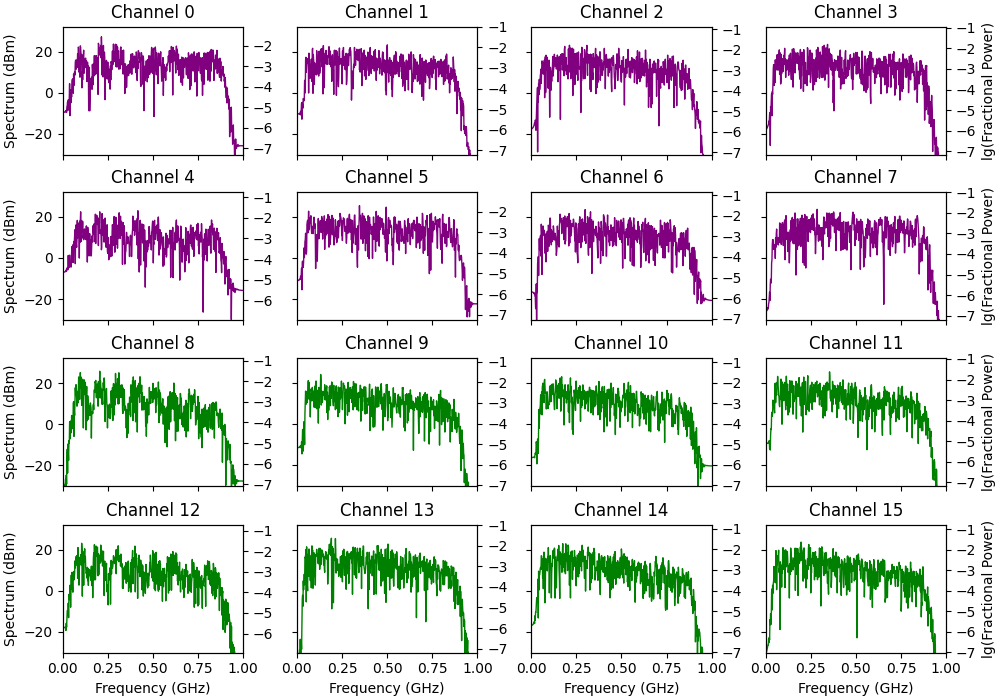
\includegraphics[width=\textwidth]{sections/5sa-cleaning/images/firstmin_station_2_run_17627_eventNo_2_spectrum.png}
      \end{subfigure}
      \caption{Example waveform (left) and spectrum (right) for an event taken within the first minute of a new run, motivating the removal of all events within the first minute of a run. This is the second event of run 17,627 of ARA2.}
      \label{fig:firstmin_waveform}
    \end{figure}
    
    % SNR or RMS vs unix time for the start of the run is not that telling. I don't remember which variables showed that the first minute of runs were bad but I'll have to remind myself
    % Myoungchul's wiki says its ADC. I'm not sure if we have anything related to ADC saved in L2 data
    % So I might have to go back to L1 data for this
    \missingfigure{2D plot showing ADC vs unixtime for the first 1 hour of a run. \label{fig:firstmin_2d}}

  \subsection{Spark Events}
  
    Another class of detector glitch backgrounds is called the Spark Event. 
    These events occur when one of the digitizing boards on the station's mainboard withstands a surge of current that inflates the digitized signal.
    Each digitizing board reads out one string for each ARA station so if one string has noticeably inflated RMS compared to the other strings, a spark event has likely taken place.
    To identify these events, the ratio in average waveform power is taken between the two strings with the greatest average power consumption. 
    Each station has a different threshold for removing an event based on this so called spark power ratio, but for ARA2 the threshold is approximately 3. 
    
    The waveform and spectrum of an example spark event is shown in Figure~\ref{fig:spark_waveform}
    
    \begin{figure}
      \centering
      \begin{subfigure}[t]{0.48\textwidth}
        \centering
        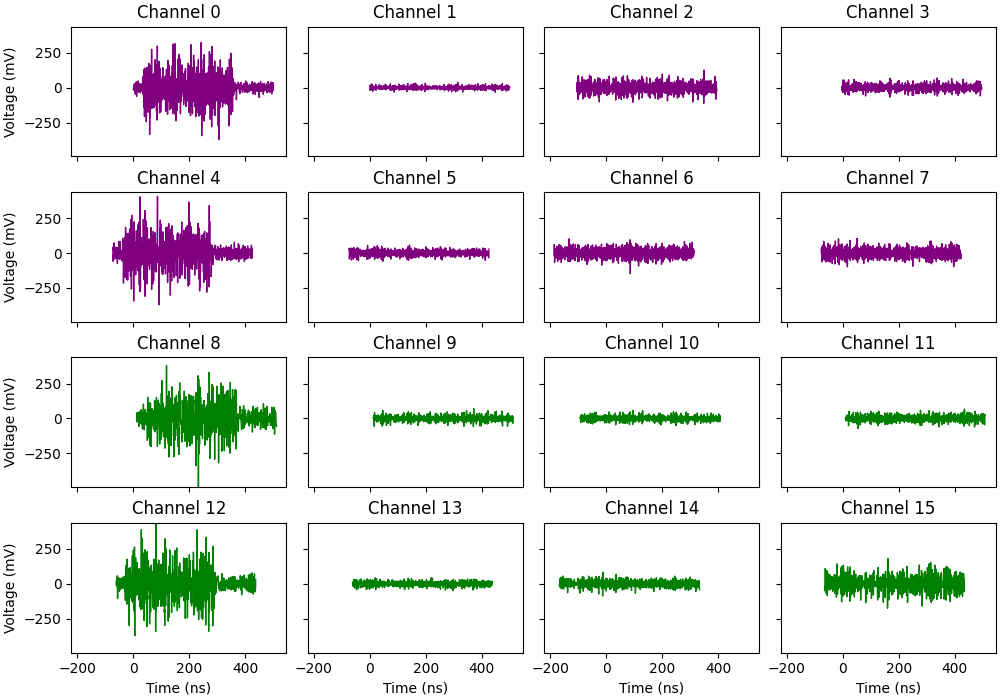
\includegraphics[width=\textwidth]{sections/5sa-cleaning/images/spark_station_2_run_7100_eventNo_1467_trace.png}
      \end{subfigure}
      ~
      \begin{subfigure}[t]{0.48\textwidth}
        \centering
        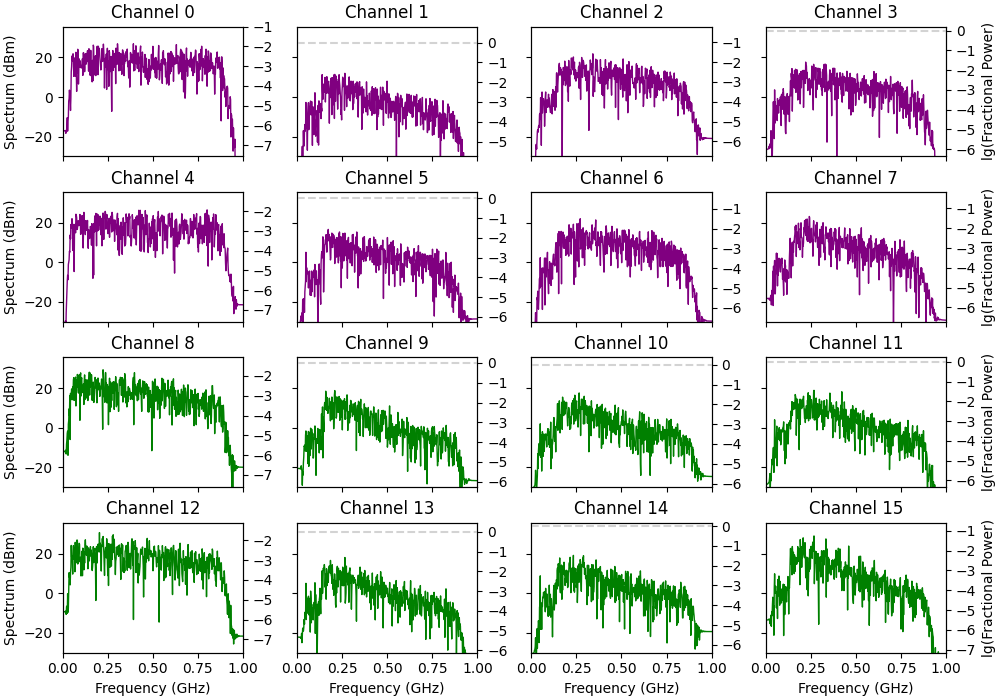
\includegraphics[width=\textwidth]{sections/5sa-cleaning/images/spark_station_2_run_7100_eventNo_1467_spectrum.png}
      \end{subfigure}
      \caption{Example waveform (left) and spectrum (right) for a spark event. Notice the significant waveform inflation in Channel 0, 4, 8, 12 (all from the same string, sharing a digitizing board) and the flattened spectrum that result from the digitizing board malfunction. This example is event 1467 of run 7100 in ARA2.}
      \label{fig:spark_waveform}
    \end{figure}

\section{Removing Anthropogenic and Science Backgrounds}

  After all erroneously digitized events are removed, events that include backgrounds we do not want to misclassify as neutrino signals must be removed. 
  This includes mis-tagged calibration pulser events, runs with known anthropogenic backgrounds, and potential cosmic ray events. 

  \subsection{Geometry Cut}
  
    The geometry cut is programmed to catch calibration pulser events that are not tagged as calibration pulser events. 
    % State how often this happens
    This may occur because the calibration pulser on a station is programmed to run once per second but it is the station's job to trigger naturally on the signals from the pulser. % Check the 1 per second bit
    The station records when the calibration pulser is firing and logs an event as a calibration event if the station triggers while the pulser is live. 
    Sometimes, calibration pulser events are not tagged as such and slip into the science dataset.
    For ARA2, events like these appear in the windows of reconstructed zenith and azimuth described in Table~\ref{tab:A2GC} on a configuration-by-configuration basis.
    The Geometry Cut enforces that events that fall within these windows are removed entirely from the analysis to remove unwanted pulser contamination from our samples.  
    
    The signals from calibration pulsers are usually recorded with strong pulses, making the interferometric reconstruction of the calpulser event obvious. 
    However pulser signals can shift in such a way that secondary solutions for the reconstruction overtake the correct solution. 
    This gives rise to populations of reconstructed calibration pulser events that are called "mirrors". 
    \missingfigure{calibration pulser mirror skymap and trace}
    \missingfigure{phi vs theta for all CP events with annotations pointing out CP5, CP5 mirror, and CP6}
    
    \begin{table}
      \centering
      \begin{tabular}{ | c | c c | c c |}
        \hline
        Object Being Cut & $\theta (^{\circ})$ & $\Delta\theta (^{\circ})$ & $\phi (^{\circ})$ & $\Delta\phi (^{\circ})$ \\
        \hline
        CP 5V & -23.5 & 4.5 & -26.35 & 4.7 \\
        CP 5V Mirror & 32.45 & 5.3 & -25.55 & 3.8 \\
        % CP 5V Mirror & 32.45 & 5.3 & -42.1 & 3.75 \\
        CP 6V & 4.5 & 5.95 & 62.9 & 6.25 \\
        \hline
      \end{tabular}
      \caption{Untagged Calibration Pulser reconstruction regions for ARA2. These cuts were inspired by the works of Myoungchul Kim from Chiba University.}
      \label{tab:A2GC}
    \end{table}
    
    To ensure that all potential untagged calibration pulser events are captured within the geometry cut, a gaussian kernel density equation is fit over the distribution of reconstructed zenith and azimuth of these events. 
    The gaussian kernel density equation was chosen by Brian Clark as the most appropriate for our data. 
    This allows us to model the tails of the reconstructed arrival directions to ensure no untagged calibration pulser events arise in our full data sample.
    
    \missingfigure{CP fits for CP5, CP5M, and CP6}
    % Should I show a plot motivating calpulser leakage? Or just cite somebody else

  \subsection{Bad Configuration Cut}
  
    Station configurations where the livetime of data, excluding bad runs, is less than 30 days are excluded from analysis. 
    Table~\ref{tab:badconfigs} shows the list of bad configurations for each station in the array. 
    Note that A2, the station focused on in this thesis, does not have any bad configurations so this cut is not applied in this thesis. 
    Due to challenges synchronizing the colocated A5 and PA instruments, A5 livetime recorded while the PA was recording are omitted to remove the possibility that duplicate events (events seen in both A5 and PA instruments) appear in the analysis. 
    Configuration 2 of A5 has more than 30 days of raw livetime, but after excluding data taken while the PA was running, A5 has less than 30 days of livetime and is therefore excluded from the analysis. 
    
    \begin{table}
      \centering
      \begin{tabular}{| c | c |}
        \hline
        Station & Bad Configurations \\
        \hline
        1 & 1 \\
        2 & None \\
        3 & None \\
        4 & 1 \\
        5 & 2 \\
        PA & 3 \\
      \end{tabular}
      \caption{Every ARA station's livetime configurations excluded from the analysis via the Bad Run Cut due to a lack of sufficient livetime. }
    \end{table}

  \subsection{Bad Run Cut}
    
    The Bad Run Cut draws directly from the Bad Run Log for the appropriate ARA station. 
    Runs are typically added to the Bad Run Log if there are known anthropogenic backgrounds present during the run. 
    This includes, but is not limited to, runs that are known to include surface pulsing calibration campaigns and heavy station activity that cannot be cleaned simply (for example, a geometry cut cannot remove snowmobile backgrounds that move in reconstructed azimuth and zenith). 
    
    Some runs can be cut due to unusual voltages in the digitizing daughter boards. \todo{explain the DDA run cut}
    Others can be cut because the station's configuration is abnormal as discussed in Section~\ref{sec:a2configs}
    
    \missingfigure{}
    
    For runs that include a large portion of anthropogenic background, it is safer to remove the entire run than to add dozens of multi-dimensional and hyper-specific cuts to remove the data. 
    The livetime reduction is not significant in doing so. 
    Brian Clark created a pipeline that systematically identifies runs with an excessive amount of outliers. 
    This pipeline takes the global maximum correlation for each RF event, plots them on a histogram, and fits two gamma Gumbel curves to the histogram. 
    The Gumbel curve is defined as % Cite Gumbel
    \begin{equation}
      f(x) = A \frac{ \beta^{\alpha} }{ \sigma ~ \Gamma(\alpha) } e^{- ( \alpha \frac{x-\mu}{\sigma} + \beta e^{({-\frac{x-\mu}{\sigma} })} ) }
      \label{eq:gumbel}
    \end{equation}
    where $A$ is a scaling factor, $\alpha=\beta$ and is initialized to 1 but free to fit, $\sigma$ is initialized as the average between the lower and upper 1$\sigma$ boundaries of the curve is called the scale parameter, and $\mu$ is initialized as peak of the histogram and called the location parameter. 
    This distribution is "suitable for modelling highly skewed and heavy-tailed data" and fits our thermal backgrounds and outliers well.  % cite http://www.kurims.kyoto-u.ac.jp/EMIS/journals/AMEN/2020/AMEN-190321.pdf and their 1st source
    The first gamma Gumbel curve is fit to the thermal background and the second is fit to the remaining outliers. 
    Examples of the gamma Gumbel curve fits to a clean and contaminated run of A2 are shown in Figure~\ref{fig:gumbel-clean} and Figure~\ref{fig:gumbel-dirty}, respectively.
    The difference between the test statistics of the Poisson negative log-likelihoods for each dual component gamma Gumbel distribution is then calculated. 
    This $\Delta TS$ parameter characterizes the separation between populations of thermal backgrounds and outliers in correlation-space. 
    A low $\Delta TS$ implies low separation and that the run is not polluted with abnormally correlated outliers. 
    A high $\Delta TS$ implies the opposite, that many events in the run are outliers in the regime of global max correlation. 
    A histogram of the $\Delta TS$ values for each run in each station's livetime configuration is plotted. 
    A run-level cut based on the value of $\Delta TS$ for the run is determined based on the presence of runs with copious outliers compared to the distribution of runs that are predominately thermal as shown in Figure~\ref{fig:deltaTS-per-config}. 
    
    \missingfigure{Gumbel for a clean run in A2 \label{fig:gumbel-clean}}
    \missingfigure{Gubmel for an outlier-y run in A2 \label{fig:gumbel-dirty}}
    \missingfigure{Distribution of gumbel curves for each config of A2 \label{fig:deltaTS-per-config}}
    
    
  \subsection{Spatio-Temporal Cut}
  
    Any anthropogenic background that is not removed by the Bad Run Cut is likely to be removed by the spatio-temporal cut. 
    
  \subsection{Zenith Cut}
  
    The Zenith Cut is employed at the end of the cleaning pipeline to remove any remaining anthropogenic surface events, such as continuous wave contaminated events that weren't fully filtered, and cosmic ray events. 
    The cosmic ray events that ARA can observe typically result from an ultra high energy cosmic ray (UHECR) interacting in the atmosphere, causing an airshower, and potentially impacting into the ice. 
    Depending on the energy and direction the UHECR is traveling in, an ARA station may see radio signals from the air shower portion and/or the ice-impacting core. 
    % Cite Nicolas, maybe show photos
    The Zenith Cut is harsh and strict and is employed last so that other cuts can be tuned as much as possible to remove backgrounds. 
    Continuous Wave contamination interferes with the reconstruction of a signal and can therefore make a surface event reconstruct in the ice. 
    Relying on the zenith cut to remove all surface related backgrounds is risky for this reason and should be employed near the end of cleaning. 
    
    We employ a conservative zenith cut at 0 degrees in elevation to ensure that all surface events are removed from the analysis. 
    
  \subsection{Low Reconstruction Confidence Cut}
    
    For the few remaining events, they are cleaned up using 
  
  % solar activity? 
  
\section{Employment of Cuts and Impact on Potential Neutrino Events}

  The cuts are applied to A2 data in the following order: 
  \begin{enumerate}
    \item Bad Run Cut
    \item Spark Event Cut
    \item Geometry Cut
    \item Spatio-Temporal Cut
    \item Zenith Cut
    \item Low Reconstruction Confidence Cut
  \end{enumerate}

  \missingfigure{For each configuration: efficiencies, snr-vs-corr for noise, neutrinos with no and all cuts, data with no and all cuts.}
  
  
  
  
  
  